
\fancyhead[C]{Section 12.5}
\fancyhead[R]{\daythree}

\iftoggle{questions}{
\begin{center}{\large \textbf{Math 2551 Worksheet: Lines and Planes}}
\end{center}


\begin{enumerate}
	
	\item Find an equation for 
	\begin{enumerate}
		\item the line through point $P=(1,2,-1)$ and point $Q=(-1,0,1)$.
		
		\item the line through $(0,-7,0)$ perpendicular to the plane $x+2y+2z=13$.
		
		\item the line in which the planes $3x-6y-2z=3$ and $2x+y-2z=2$ intersect.
	\end{enumerate}
	
	\item Find a vector in the direction of the line of intersection $\ell$ of the planes $2x+y-z=3$ and  $x+2y+z=2.$  Find a plane which goes	through $(2,1,-1)$ and is perpendicular to $\ell$ (and thus both planes).  
	
	\item Find 2 planes that are not parallel that both contain the points $P(1,-1,1)$, $Q(3,2,0)$, and $R(5,5,-1)$. When will 3 distinct points NOT determine a unique plane? 
	
	\item Find the point where the line $\br(t)=\langle 2, 3+2t, 1+t\rangle$  intersects the plane
	$2x-y+3z=6$.
	
	\item  %12.5 68
	How can you tell when two planes $A_1x + B_1 y + C_1 z = D_1$ and  $A_2x + B_2 y + C_2 z = D_2$ are parallel?  Perpendicular?
	Justify your answer. 
	
	\item Find the point at which the lines $\ell_1(t)=\langle 
	2,3,1\rangle+\langle 1,-1,1\rangle t$ and $\ell_2(t)=\langle 2,1,-2\rangle 
	t+\langle 6,2,1\rangle$ intersect.
	
%	\item Recall from linear algebra that the \textbf{projection} of a vector 
%$\bu$ onto $\bv$ is the component of $\bu$ in the direction of $\bv: 
%\proj_{\bv}\bu=\dfrac{\bu\cdot\bv}{|\bv|^2}\bv$.
%	
%	\begin{enumerate}
%		\item The distance from a point $P$ to a plane is the shortest distance 
%from $P$ to any point on the plane.  Use this and the above to compute the 
%distance from the point $P=(1,2,3)$ to the plane $2x-y+3z=5$.\\
%		
%		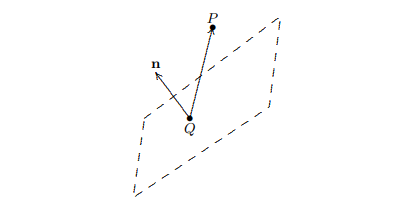
\includegraphics[scale=0.6]{12_5_plane_dist.png}
%		
%		\item The distance from a point $P$ to a line is the shortest distance 
%from $P$ to any point on the line.  Use this and a well-chosen cross product 
%to 
%compute the distance from the point $P=(-1,2,1)$ to the line $\langle 
%1,1,1\rangle+t\langle 2,3,-1\rangle$.\\
%		
%		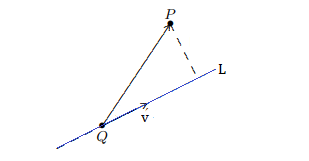
\includegraphics[scale=0.7]{12_5_line_dist.png}
%	\end{enumerate}

\end{enumerate}
}{}

\iftoggle{answers}{
\begin{center}{\large \textbf{Math 2551 Worksheet Answers: Lines and Planes}}
\end{center}


\begin{enumerate}
	
	\item 
	\begin{enumerate}
		\item $\br(t)=\langle 1 -2t, 2-2t, -1+2t\rangle$
		
		\item $\br(t)=\langle t, -7+2t,2t\rangle$
		
		\item $\br(t)=\langle 1+14t, 2t, 15t\rangle$
	\end{enumerate}
	
	\item vector: $3\bi-3\bj+3\bk$.
	
	plane: $3(x-2)-3(y-1)+3(z+1)=0$
	
	\item many correct solutions; pick two distinct points off of the line $PQ$ which are not collinear with the given points.  Two such planes are $-2(x-1)+3(y+1)+5(z-1)=0$ and $-3(x-1)+3(y+1)+3(z-1)=0$.
	
	\item $(2,7,3)$
	
	\item  Parallel: $\langle A_1, B_1, C_1\rangle = \lambda \langle A_2, B_2, C_2\rangle$ for some $\lambda\neq 0$
	
	Perpendicular:  $\langle A_1, B_1, C_1\rangle \dotp \langle A_2, B_2, C_2\rangle=0$
	
	\item $(4,1,3)$
%	\item \begin{enumerate}
%		\item distance $= \dfrac{\vec{QP}\cdot\bn}{\bn}$ with $Q=(1,0,1)$ (any 
%point on the plane works).  So the distance is $\dfrac{\langle 
%0,2,2\rangle\cdot\langle2,-1,3\rangle}{|\langle 
%2,-1,3\rangle|}=\dfrac{4}{\sqrt{14}}$
%		
%		\item distance is $|\vec{QP}|\sin(\theta)=\dfrac{|\vec{QP}\times 
%\bv|}{|\bv|}$ where $Q=(1,1,1), \bv=\langle 2,3,-1\rangle$ (any point on the 
%line and any direction vector works). So the distance is 
%$\dfrac{\sqrt{69}}{\sqrt{14}}$.
%	\end{enumerate}
\end{enumerate}
}{}
\iftoggle{solutions}
{
Solutions go here in the same format.
}{}
